\documentclass{uebblatt}

\usepackage{ifthen,tikz}

\makeatletter
\newcommand\binomialCoefficient[2]{%
    % Store values 
    \c@pgf@counta=#1% n
    \c@pgf@countb=#2% k
    %
    % Take advantage of symmetry if k > n - k
    \c@pgf@countc=\c@pgf@counta%
    \advance\c@pgf@countc by-\c@pgf@countb%
    \ifnum\c@pgf@countb>\c@pgf@countc%
        \c@pgf@countb=\c@pgf@countc%
    \fi%
    %
    % Recursively compute the coefficients
    \c@pgf@countc=1% will hold the result
    \c@pgf@countd=0% counter
    \pgfmathloop% c -> c*(n-i)/(i+1) for i=0,...,k-1
        \ifnum\c@pgf@countd<\c@pgf@countb%
        \multiply\c@pgf@countc by\c@pgf@counta%
        \advance\c@pgf@counta by-1%
        \advance\c@pgf@countd by1%
        \divide\c@pgf@countc by\c@pgf@countd%
    \repeatpgfmathloop%
    \the\c@pgf@countc%
}
\makeatother

\newcommand{\pascaltriangle}{
  \newdimen\R
  \R=.4cm
  \newcommand\mycolor{gray}
  \begin{tikzpicture}[line width=.8pt]
    \foreach \k in {0,...,12}{
      \begin{scope}[shift={(-60:{sqrt(3)*\R*\k})}]
	\pgfmathtruncatemacro\ystart{12-\k}
	\foreach \n in {0,...,\ystart}{
	  \pgfmathtruncatemacro\newn{\n+\k}
	  %\ifthenelse{\k=0}{\def\mycolor{pink}}{}
	  %\ifthenelse{\k=1}{\def\mycolor{yellow}}{}
	  %\ifthenelse{\k=2}{\def\mycolor{blue}}{}
	  %\ifthenelse{\k=3}{\def\mycolor{green}}{}
	  %\ifthenelse{\k=8 \AND \n < 4}{\def\mycolor{purple}}{}
	  %\ifthenelse{\k=9 \AND \n = 3}{\def\mycolor{purple}}{}
	  \begin{scope}[shift={(-120:{sqrt(3)*\R*\n})}]
	     \draw[top color=\mycolor!3,bottom color=\mycolor!10] 
	       (30:\R) \foreach \x in {90,150,...,330} {
		  -- (\x:\R)}
		  -- cycle (90:0)
		     node {\tiny $\mathbf{\binomialCoefficient{\newn}{\k}}$};
	   \end{scope}
	}
      \end{scope}
    }
  \end{tikzpicture}
}

% Taken from Todd Lehman (CC-BY-SA) at https://tex.stackexchange.com/a/44920/32372

\newcommand{\setisprime}[1]{
  % Sets \isprime based on #1.
  \ifnum#1=1 \gdef\isprime{0} \else \gdef\isprime{1} \fi
  \foreach \sip in {2, 3,5,...,#1} {
    \pgfmathparse{\sip*\sip>#1? 1:0}
    \ifthenelse{\pgfmathresult=1}{
      % Early-out if \sip^2 > #1.
      \breakforeach
    }{
      % Otherwise test if \sip divides #1.
      \pgfmathparse{Mod(#1,\sip)==0? 1:0}
      \ifthenelse{\pgfmathresult=1}{
        \gdef\isprime{0}
        \breakforeach
      }{}
    }
  }
}

\newcommand{\setxy}[1]{
  % Sets \x and \y to loction of cell #1.
  \pgfmathtruncatemacro{\x}{Mod(#1-1,\cols)}
  \pgfmathtruncatemacro{\y}{(#1-1) / \cols}
  \pgfmathtruncatemacro{\y}{\cols - 1 - \y}
  \pgfmathparse{2.5*(\x+.5)}\let\x\pgfmathresult
  \pgfmathparse{2.5*(\y+.5)}\let\y\pgfmathresult
}

\newcommand{\numlabel}[2]{
  % Draws label #2 at cell #1.
  \setxy{\n}
  \node[fill=none, text=black] at (\x,\y) {#2};
}

\newcommand{\drawpolygon}[2]{
  % Draws polygon with #2 vertexes at cell #1.
  \setxy{#1}
  \ifthenelse{#2>1}{ % Polygon must have at least 2 sides.
    \ifthenelse{#2<30}{ % Draw polygon if it has a small number of sides.
      \filldraw (\x,\y) +(90:1)
      \foreach \drawi in {1,...,#2} {-- +(\drawi/#2*360+90:1)} -- cycle;
    }{ % Else approximate with circle.
      \filldraw (\x,\y) circle(1);
    }
  }{}
}

\newcommand{\setpolygoncolor}[1]{
  % Sets color based on #1.
  \gdef\polycolor{black}
  \ifnum#1=2\gdef\polycolor{black!50!white}\fi
  \ifnum#1=3\gdef\polycolor{yellow!95!red}\fi
  \ifnum#1=5\gdef\polycolor{yellow!0!red}\fi
  \ifnum#1=7\gdef\polycolor{blue!75!green}\fi
  \ifnum#1=11\gdef\polycolor{blue!70!red}\fi
  \ifnum#1=13\gdef\polycolor{blue!40!red}\fi
  \ifnum#1=17\gdef\polycolor{green!50!blue}\fi
  \ifnum#1=19\gdef\polycolor{green!80!black}\fi
  \ifnum#1=23\gdef\polycolor{green!50!red}\fi
  \ifnum#1=29\gdef\polycolor{yellow!50!black}\fi
  \ifnum#1=31\gdef\polycolor{orange!50!black}\fi
  \ifnum#1=37\gdef\polycolor{red!50!black}\fi
  \ifnum#1=41\gdef\polycolor{purple!50!black}\fi
  \ifnum#1=43\gdef\polycolor{blue!50!black}\fi
  \ifnum#1=47\gdef\polycolor{green!50!black}\fi
  \ifnum#1=53\gdef\polycolor{white!50!black}\fi
  \ifnum#1=59\gdef\polycolor{white!50!black}\fi
  \ifnum#1=61\gdef\polycolor{white!50!black}\fi
  \ifnum#1=67\gdef\polycolor{white!50!black}\fi
}

\newcommand{\sieve}[2]{
  \def\cols{#1}
  \def\rows{#2}
  \begin{tikzpicture}[scale=.5]
  \pgfmathtruncatemacro{\nmax}{\rows * \cols}

  \foreach \n in {1,...,\nmax} {
    \begin{scope}[fill=gray, fill opacity=.05,
                  draw=gray, draw opacity=.10,
                  line width=4]
      \drawpolygon{\n}{\n}
    \end{scope}
    \setisprime{\n}
    \ifthenelse{\isprime=1}{
      \numlabel{\n}{\textbf{\n}}
    }{
      \def\startintensity{.33}
      \def\incrintensity{.10}
      \def\intensity{\startintensity}

      \def\m{\n}
      \pgfmathtruncatemacro{\i}{\m / 2}

      % Divide \m by \i until \m is extinguished.
      % Increment \i each time it does not divide into \m.
      \whiledo{\m>1}{
        \setisprime{\i}
        \pgfmathparse{Mod(\m,\i)==0? 1:0}
        \ifthenelse{\pgfmathresult=1\and\isprime=1}{
          \setpolygoncolor{\i}
          \begin{scope}[fill=\polycolor, fill opacity=\intensity,
                        draw=\polycolor!85!black, draw opacity=\intensity,
                        line width=\intensity*1.5]
            \drawpolygon{\n}{\i}
          \end{scope}
          \pgfmathtruncatemacro{\m}{\m / \i}
          \pgfmathparse{\intensity + \incrintensity}\let\intensity\pgfmathresult
        }{
          \pgfmathtruncatemacro{\i}{\i - 1}
          \def\intensity{\startintensity}
        }
      }
      \begin{scope}[text=black, text opacity=.5]
        \numlabel{\n}{\scriptsize\n}
      \end{scope}
    }
  }

  \end{tikzpicture}
}

\newcommand{\fakesieve}[2]{
  \def\cols{#1}
  \def\rows{#2}
  \begin{tikzpicture}[scale=.5,opacity=0]
  \pgfmathtruncatemacro{\nmax}{\rows * \cols}

  \foreach \n in {1,...,\nmax} {
    \begin{scope}[fill=gray,
                  draw=gray,
                  line width=4]
      \drawpolygon{\n}{\n}
    \end{scope}
    \setisprime{\n}
    \ifthenelse{\isprime=1}{
      \numlabel{\n}{\bf\n}
    }{
      \def\startintensity{.33}
      \def\incrintensity{.10}
      \def\intensity{\startintensity}

      \def\m{\n}
      \pgfmathtruncatemacro{\i}{\m / 2}

      % Divide \m by \i until \m is extinguished.
      % Increment \i each time it does not divide into \m.
      \whiledo{\m>1}{
        \setisprime{\i}
        \pgfmathparse{Mod(\m,\i)==0? 1:0}
        \ifthenelse{\pgfmathresult=1\and\isprime=1}{
          \setpolygoncolor{\i}
          \begin{scope}[fill=\polycolor,
                        draw=\polycolor!85!black,
                        line width=\intensity*1.5]
            \drawpolygon{\n}{\i}
          \end{scope}
          \pgfmathtruncatemacro{\m}{\m / \i}
          \pgfmathparse{\intensity + \incrintensity}\let\intensity\pgfmathresult
        }{
          \pgfmathtruncatemacro{\i}{\i - 1}
          \def\intensity{\startintensity}
        }
      }
      \begin{scope}[text=black]
        \numlabel{\n}{\scriptsize\n}
      \end{scope}
    }
  }

  \end{tikzpicture}
}

\pagestyle{empty}

\AddToHook{shipout/background}{%
  \put(0in,-\paperheight){
\includegraphics[width=\paperwidth]{fr1}}%
}

\begin{document}

\begin{blatt}{Primzahlen}

\begin{aufgabe}{Die Mysterien der Ulam-Spirale}
\begin{wrapfigure}{r}{4cm}
\vspace*{-1.5cm}
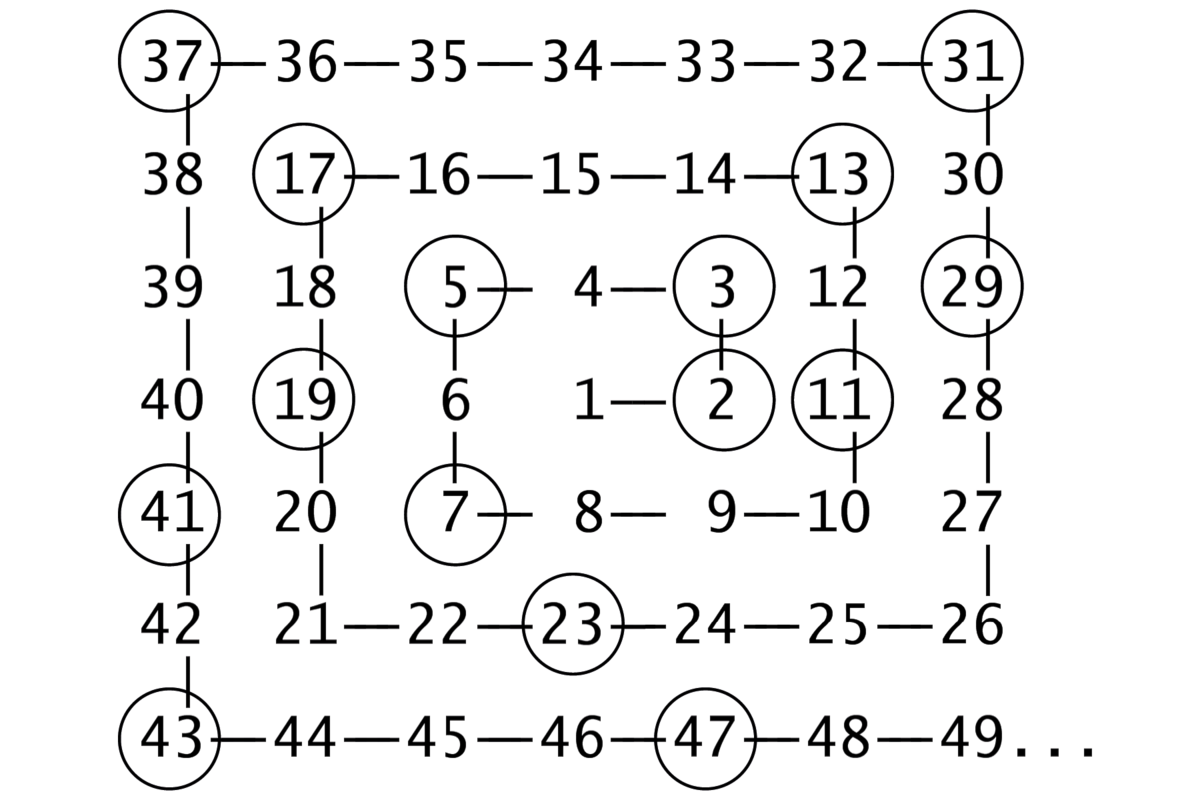
\includegraphics[width=6cm]{ulam}
\end{wrapfigure}
Rechts abgebildet ist der Beginn der \emph{Ulam-Spirale}. 
\begin{enumerate}
\item Vielleicht macht es dir Spaß, sie weiter zu zeichnen. Primzahlen häufen
sich an den Diagonal- und Querachsen.
\item Was passiert, wenn du statt der~$1$ die~$41$ als Ausgangspunkt nimmst?
\end{enumerate}
\end{aufgabe}

\begin{aufgabe}{Ein verstecktes Fraktal im Pascalschen Dreieck}
\begin{enumerate}
\item Die Grafik zeigt die ersten 12 Zeilen des sog. Pascalschen Dreiecks. Nach
welchem Bildungsprinzip ergeben sich die Zahlen?
\item Färbe alle Vielfachen der Zahl~2 ein. Was stellst du fest?
\item Ein ähnliches Fraktal ergibt sich, wenn man die Vielfachen einer anderen
Primzahl einfärbt. Probiere es aus.
\end{enumerate}
\centering\pascaltriangle
\end{aufgabe}

\enlargethispage{2em}
\begin{aufgabe}{Das Sieb des Eratosthenes}
Vielleicht macht es dir Spaß, das \emph{Sieb des Eratosthenes} länger als
abgebildet durchzuführen. Eine gute Anleitung gibt der Wikipedia-Artikel zu
diesem Thema.
\smallskip

\centering
\scalebox{0.8}{\sieve{10}{6}}
\end{aufgabe}

\begin{aufgabe}{Lucas--Lehmer-Test in Aktion}
Die Lucas--Lehmer-Zahlenfolge ist folgende unendliche Zahlenfolge:
\[ 4,\quad 14,\quad 194,\quad 37634,\quad 1416317954,\quad \ldots \]
Die jeweils nächste Zahl ist zwei weniger als das Quadrat der vorherigen: $s_{n+1} = s_n^2 - 2$.
Der \emph{LL-Rest} einer Mersenne-Zahl~$2^p-1$ ist der Rest bei Division
der~$(p-1)$-ten Lucas--Lehmer-Zahl durch~$2^p-1$. Zum Beispiel:
\begin{itemize}
\item Der LL-Rest von~$2^3 - 1 = 7$ ist der Divisionsrest bei~$14 :
7$, also Null.
\item Der LL-Rest von~$2^4 - 1 = 15$ ist der Divisionsrest bei~$194
: 15$, also~$14$ (da~$194 = 12 \cdot 15 + 14$).
\item Der LL-Rest von~$2^5 - 1 = 31$ der Divisionsrest bei~$37634 :
31$, also Null (da $37634 = 31 \cdot 1214$).
\end{itemize}
Dass die LL-Reste von~$7$ und~$31$ jeweils Null sind, ist kein Zufall:
\emph{Ist~$p$ eine ungerade Primzahl, so ist die Zahl~$2^p - 1$ dann und nur
dann ebenfalls prim, wenn ihr LL-Rest Null ist.}
\begin{enumerate}
\item Was ist der~LL-Rest von~$2^6 - 1 = 63$?
\item Verwende den LL-Test, um zu prüfen, ob~$2^{11} - 1 = 2047$ prim ist.
\end{enumerate}
\end{aufgabe}

\begin{aufgabe}{Beliebig große Lücken zwischen Primzahlen}
Zeige: Zu jeder Lauflänge~$n \geq 1$ gibt es eine Folge von~$n$ direkt
aufeinanderfolgenden Zahlen, welche alle keine Primzahlen sind.

Mit anderen Worten: Irgendwo auf dem Zahlenstrahl gibt es fünf
aufeinanderfolgende Zahlen, die alle keine Primzahlen sind; irgendwo anders
gibt es hundert aufeinanderfolgende Zahlen, die alle keine Primzahlen sind; und
so weiter.

{\scriptsize\emph{Tipp.} Kannst du den Zahlen~$m! + 2$ bis~$m! + m$ ansehen, welche Teiler
sie auf jeden Fall haben? Dabei ist~$m! = m \cdot (m-1) \cdot \ldots
\cdot 2 \cdot 1$ (gesprochen: "`$m$ Fakultät"').\par}
\end{aufgabe}

\begin{aufgabe}{Primzahlen mögen die 6 und die 24}
\begin{enumerate}
\item Zeige: Jede Primzahl größer als~$3$ liegt benachbart zu einem Vielfachen
von~$6$. Mit anderen Worten: Ist~$p > 3$ eine Primzahl, so~$6 \mid p - 1$
oder~$6 \mid p + 1$.

{\scriptsize\emph{Tipp.} Eine Zahl ist genau dann ein Vielfaches von~$6$, wenn sie ein
Vielfaches von~$2$ und von~$3$ ist. Weißt du von den drei Zahlen~$p-1$,~$p$
und~$p+1$, ob sie ein Vielfaches von~$3$ sind?\par}

\item Sei~$p$ eine beliebige Primzahl größer als~$3$.
Zeige: Die Zahl~$p^2 - 1$ ist ein ganzzahliges Vielfaches von~$24$.
(In anderen Worten: $24 \mid p^2 - 1$.)
\end{enumerate}
\end{aufgabe}

\begin{aufgabe}{Zusammengesetzte Mersenne-Zahlen}
Positive Zahlen, die nicht Primzahlen sind, heißen \emph{zusammengesetzte
Zahlen}. Zeige: Ist~$n$ eine zusammengesetzte Zahl, so ist die
Mersenne-Zahl~$2^n - 1$ ebenfalls zusammengesetzt. (In der Folge hat~$2^n - 1$
also nur dann eine Chance, prim zu sein, wenn~$n$ selbst prim ist. Das heißt
aber nicht, dass in diesem Fall~$2^n-1$ sicher prim ist.)

{\scriptsize\emph{Tipp.} Beginne deine Überlegungen mit der Feststellung,
dass sich~$n$ als~$n = ab$ für gewisse Faktoren~$a$ und~$b$ schreiben lässt.
Nutze dann die \emph{Formel für die geometrische Reihe}: Für jede Zahl~$q$
gilt~$q^k - 1 = (q - 1) \cdot (1 + q + q^2 + \ldots + q^{k-1})$. Dies ist eine
von einer kleinen Handvoll Formeln, die die meisten Mathematiker*innen
auswendig kennen.\par}
\end{aufgabe}

\newpage
\begin{aufgabe}{Charakterisierung gerade perfekter Zahlen}
Eine positive natürliche Zahl heißt genau dann \emph{perfekt}, wenn sie gleich
der Summe ihrer echten Teiler ist. Etwa sind die Zahlen~$6$ und~$28$ perfekt,
denn~$6 = 1 + 2 + 3$ und~$28 = 1 + 2 + 4 + 7 + 14$. Für die Mersenne-Zahl~$q =
2^2 - 1 = 3$ gilt~$6 = q (q+1) / 2$ und für die Mersenne-Zahl~$q = 2^3 - 1 = 7$
gilt~$28 = q (q+1) / 2$. Das ist kein Zufall: Es ist nämlich ein Theorem, dass
wenn~$q = 2^{n+1} - 1$ eine beliebige Mersenne-Zahl ist, die Zahl~$N = q (q+1) / 2$
gerade und perfekt ist.
\begin{enumerate}
\item Verifiziere: In dieser Situation gilt~$q (q+1) / 2 = 2^n \cdot (2^{n+1} - 1)$.
(Damit ist also~$N$ gerade.)
\item Die Grafik zeigt einen grafischen Beweis, dass~$N$ perfekt ist. Vollziehe
ihn nach.
\end{enumerate}
Übrigens: Es gilt auch die Umkehrung -- jede gerade perfekte Zahl ist von der
hier vorgestellten Form.

\centering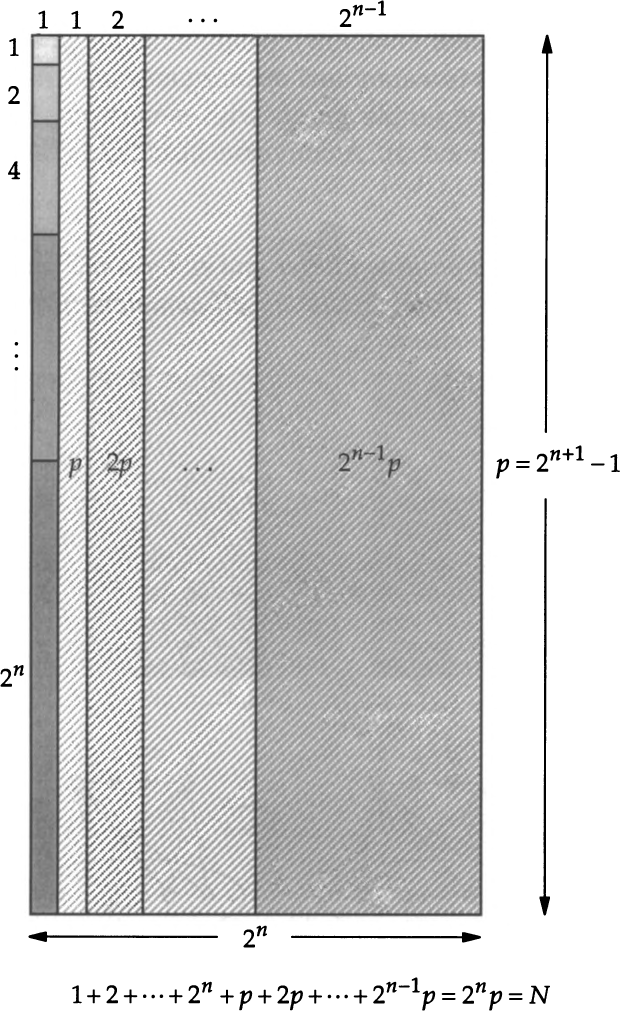
\includegraphics[height=15cm]{mersenne-perfekt}
\end{aufgabe}

\begin{aufgabe}{Eine stumpfe obere Schranke an die Größen von Primzahlen}
Euklid bewies die Unendlichkeit der Primzahlen wie folgt:
\begin{quote}
\emph{Sind Primzahlen~$p_1,\ldots,p_n$ gegeben, so hat die Zahl~$p_1 \cdot p_2 \cdot \ldots \cdot p_n
+ 1$ wie jede natürliche Zahl, die mindestens~2 ist, irgendwelche Primfaktoren
-- aber die gegebenen Primzahlen~$p_1,\ldots,p_n$ können das nicht sein, also
sind diese Primfaktoren neue Primzahlen.}
\end{quote}
Sei im Folgenden~$p_1 = 2$ die erste Primzahl, $p_2 = 3$ die zweite und so
weiter.
\begin{enumerate}
\item Zeige: Für die~$(r+1)$-te Primzahl gilt die Abschätzung
$p_{r+1} \leq p_1 \cdots p_r + 1$.
\item Folgere mit vollständiger Induktion für alle natürlichen Zahlen~$r \geq 1$: $p_r < 2^{(2^r)}$.

{\scriptsize\emph{Tipp.} Verwende, dass für alle Zahlen~$m \geq 2$ gilt: $m/4 +
1 \leq m$. Verwende außerdem die Formel~$2^1 + 2^2 + \cdots + 2^k = 2^{k+1} -
2$.\par}
\end{enumerate}
\end{aufgabe}

\end{blatt}

\end{document}
